\documentclass[10pt, a4paper]{article}
\usepackage[paper=a4paper, left=1.5cm, right=1.5cm, bottom=1.5cm, top=3.5cm]{geometry}
\usepackage[utf8]{inputenc}
\usepackage[T1]{fontenc}
\usepackage[spanish]{babel}
\usepackage{indentfirst}
\usepackage{fancyhdr}
\usepackage{latexsym}
\usepackage{lastpage}
\usepackage[colorlinks=true, linkcolor=black]{hyperref}
\usepackage{calc}
\usepackage{a4wide}
\usepackage{listings}
\lstset{language={C++}, basicstyle=\small}
\usepackage{algorithm}
\usepackage{algorithmic}[1]
\usepackage[spanish]{babel}
\usepackage{graphicx}
\usepackage{tikz}
\usepackage{epsf}
\usepackage{amsmath}
\usepackage{framed}
\usepackage{amsfonts}
\usepackage{tkz-berge}
\usepackage{amsfonts}
\usepackage{color}
\usepackage{caratula}
\usepackage{cite}
\usepackage{paralist}


\definecolor{gray97}{gray}{.97}
\definecolor{gray75}{gray}{.75}
\definecolor{gray45}{gray}{.45}
%
% \lstset{ frame=Ltb,
% framerule=0pt,
% aboveskip=0.5cm,
% framextopmargin=3pt,
% framexbottommargin=3pt,
% framexleftmargin=0.4cm,
% framesep=0pt,
% rulesep=.4pt,
% backgroundcolor=\color{gray97},
% rulesepcolor=\color{black},
% %
% stringstyle=\ttfamily,
% showstringspaces = false,
% basicstyle=\small\ttfamily,
% commentstyle=\color{gray45},
% keywordstyle=\bfseries,
% %
% numbers=left,
% numbersep=15pt,
% numberstyle=\tiny,
% numberfirstline = false,
% breaklines=true,
% }
% % minimizar fragmentado de listados
% \lstnewenvironment{listing}[1][]
% {\lstset{#1}\pagebreak[0]}{\pagebreak[0]}
% \lstdefinestyle{consola}
% {basicstyle=\scriptsize\bf\ttfamily,
% backgroundcolor=\color{gray75},
% }
%
% \hypersetup{
%  pdfstartview= {FitH \hypercalcbp{\paperheight-\topmargin-1in-\headheight}},
%  pdfauthor={Grupo},
%  pdfsubject={Dise\~{n}o}
% }
%
% \parskip=5pt
%
% \let\olditemize\itemize
% \def\itemize{\olditemize\itemsep=0pt}
%
% \pagestyle{fancy}
% \thispagestyle{fancy}
% \addtolength{\headheight}{1pt}
% \lhead{M\'etodos Numericos}
% \cfoot{\thepage}
% \renewcommand{\footrulewidth}{0.4pt}

\setcounter{tocdepth}{5}


\begin{document}

\begin{figure}[ptb]

\includegraphics[scale=0.30]{logo.jpg}\hspace{6cm}

\includegraphics[scale=0.90]{logo_dc.jpg}
\end{figure}

%Datos de la caratula
\materia{Sistemas Operativos}
\titulo{Trabajo pr\'actico 1}
\subtitulo{Scheduling}
\hspace{6cm}
\integrante{Acosta, Javier Sebastian}{338/11}{acostajavier.ajs@gmail.com}
\integrante{Gomez, Fernando Nahuel}{695/11}{fernando.gmz12@gmail.com}
\integrante{Russo, Christian Sebastián}{679/10}{christian.russo@gmail.com}

\palabrasClave{Scheduling}
  % Reconocimiento caras. PCA. Power Method. Deflation. Autovalores. Autovectores. Matriz
  % semi definida positiva.

% \resumen{El presente trabajo analiza los algor\'itmos de resoluci\'on de sistemas de ecuaciones %
% Gauss y LU mediante una simulaci\'on del c\'alculo de Isotermas en hornos industriales. \\ %
% Expone un sistema de ecuaciones para detectar la Isoterma de 500 grados y analiza el
% comportamiento de cada algoritmo en funci\'on a la discretizaci\'on de los puntos dentro del
% horno, cantidad de instancias a resolver y variaci\'on de instantes.\\ % Finalmente, detalla las
% conclusiones obtenidas mediante la comparaci\'on de ambos algoritmos en las circunstancias
% mencionadas.\\
% }
\hypersetup{%
 % Para que el PDF se abra a página completa.
 pdfstartview= {FitH \hypercalcbp{\paperheight-\topmargin-1in-\headheight}},
 pdfauthor={Acosta, Gomez, Russo},
 pdfsubject={TP1}
}

\parskip=5pt % 10pt es el tamaño de fuente

% Pongo en 0 la distancia extra entre ítemes.
\let\olditemize\itemize
\def\itemize{\olditemize\itemsep=0pt}

% Acomodo fancyhdr <- Creo que es el encabezado de pagina
\pagestyle{fancy}
\thispagestyle{fancy}
\addtolength{\headheight}{1pt}
\lhead{Acosta, Gomez, Russo}
\rhead{2$^{do}$ Cuatrimestre 2014}
\cfoot{\thepage}
\renewcommand{\footrulewidth}{0.4pt}




%Pagina de titulo e indice
\thispagestyle{empty}

\maketitle
\tableofcontents

\newpage

	

\newcommand{\cod}[1]{{\tt #1}}
\newcommand{\negro}[1]{{\bf #1}}
\newcommand{\ital}[1]{{\em #1}}
\newcommand{\may}[1]{{\sc #1}}
\newcommand{\tab}{\hspace*{2em}}

\newenvironment{myindentpar}[1]
{\begin{list}{1}
         {\setlength{\leftmargin}{#1}}
         \item[]
}
{\end{list} }

\section{Pregunta 1}

\subsection{Enunciado del Problema:}
Programar un tipo de tarea TaskConsola, que simular\'a una tarea interactiva. La tarea debe realizar n llamadas bloqueantes, cada una de una duracion al azar1 entre bmin y bmax (inclusive). La tarea debe recibir tres parametros: n, bmin y bmax (en ese orden) que serian interpretados como los tres elementos del vector de enteros que recibe la funciion.

\subsection{Pseudocodigo}

\begin{algorithm}[H]
\caption{TaskConsola(pid, params)}
\label{pseudo:TaskConsola}
\begin{algorithmic}

\STATE n = params[0]
\STATE bmin = params[1]
\STATE bmax = params[2]
\FOR{$i=0$ hasta $n$}
    \STATE uso\_IO(pid, bmin + rand() \% (bmax - bmin +1))
\ENDFOR

\end{algorithmic}
\end{algorithm}

\subsection{Explicacion}

Para realizar una llamada \textbf{bloqueante} hacemos uso de la funcion uso\_IO, para utilizar la entrada y salida. Hacemos un ciclo que ejecuta \textbf{n} veces la funcion con el parametro de duracion al azar en el intervalo dado.
Tambien registramos nuestra nueva tarea en task\_init().

\section{Pregunta 2}

\subsection{Enunciado del Problema:}

Escribir un lote de 3 tareas distintas: una intensiva en CPU y las otras dos de tipo interactivo (TaskConsola). Ejecutar y graficar la simulacion usando el algoritmo FCFS para 1, 2 y 3 nucleos.

\subsection{Lote}
\begin{framed}

@2

TaskCPU 10

@5 

TaskConsola 9 1 7

@3

TaskConsola 4 1 5


\end{framed}


\subsection{Resultados}

\begin{figure}[H]
\begin{center}
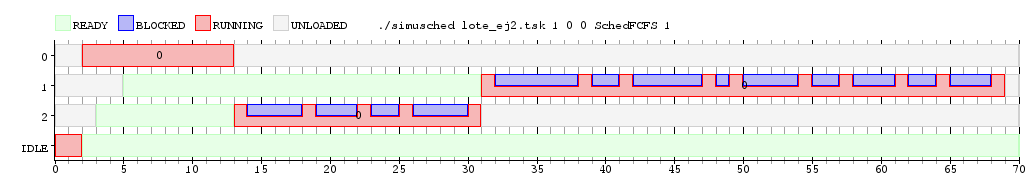
\includegraphics[width=1.1\textwidth]{img/ej2_1.png}
     \caption{FCFS con 1 núcleo}
\end{center}
\end{figure}

\textbf{Conclusiones:} Se puede ver claramente que se ejecutan las tareas de forma FCFS, es decir primero se ejecuta el proceso 0 ya que es el primero en llegar (2 unidades de tiempo) una vez finalizado se pasa la ejecucion al proceso 2 (que llego en 3 unidades de tiempo), este ejecuta las 4 llamadas bloquenates y finalmente se pasa la ejecucion al proceso 1 que fue el ultimo en llegar (5 unidades de tiempo) ejecutando las 9 llamadas bloquentes. Tambien se puede ver a simple vista que las llamadas bloqueantes, respetan el bmin y bmax


\begin{figure}[H]
\begin{center}
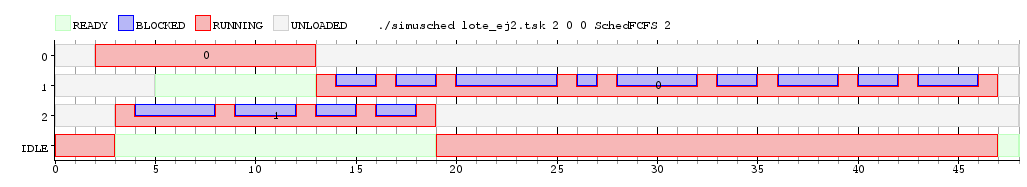
\includegraphics[width=1.1\textwidth]{img/ej2_2.png}
     \caption{FCFS con 2 núcleos}
\end{center}
\end{figure}

\textbf{Conclusiones:} En este experimento se puede ver que el funcionamiento es similar al experimento anterior, la única diferencia es que mientras se ejecuta el proceso 0, es decir cuando llega el proceso 2, al haber dos núcleos este no espera a la finalizacion del proceso 0 sino que arranca directamente su ejecución en el otro núcleo. Finalmente el proceso 1 (el restante) se ejecuta en el núcleo 0 cuando el proceso 0 (que es el primero en terminar) termina (es decir, se libera un núcleo).


\begin{figure}[H]
\begin{center}
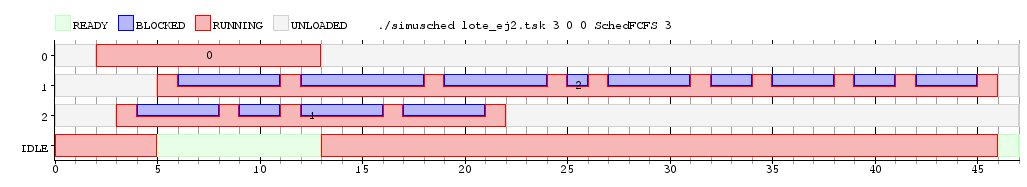
\includegraphics[width=1.1\textwidth]{img/ej2_3.png}
     \caption{FCFS con 3 núcleos}
\end{center}
\end{figure}

\textbf{Conclusiones:} Idéntico al caso anterior, pero con diferencia de que ahora tenemos tres núcleos y, por lo tanto, al haber solo 3 procesos, ninguna tiene que esperar a que otro termine, ya que cada uno puede correr en un núcleo distinto. Es por ese motivo que cada proceso se ejecuta en el instante en que llega.















\section{Pregunta 3}

\subsection{Enunciado del Problema:}

Completar la implementacion del scheduler Round-Robin implementando los metodos de la clase SchedRR en los archivos sched rr.cpp y sched rr.h. La implementacion recibe como primer parametro la cantidad de nucleos y a continuacion los valores de sus respectivos quantums. Debe utilizar una unica cola global, permitiendo asi la migracion de procesos entre nucleos.
\subsection{Pseudocodigo}

Para este ejercicio manejamos una cola q en la cual tenemos todos los procesos ready.




\begin{algorithm}[H]
\caption{SchedRR(Vector<int> argn)}
\label{pseudo:load}
\begin{algorithmic}

\STATE cantCores = argn[0]
\STATE cpuQuantum = Vector<int> de tamaño cantCores y cero en todas las posiciones.
\STATE quantumActual = Vector<int> de tamaño cantCores y cero en todas las posiciones.
\FOR{($i=0$ hasta $cantCores$)}
	\STATE quantumActual[i] = argn[i+2]
	\STATE cpuQuantum[i] = argn[i+2]	
\ENDFOR

\end{algorithmic}
\end{algorithm}




\begin{algorithm}[H]
\caption{load(pid)}
\label{pseudo:load}
\begin{algorithmic}

\STATE q.push(pid)

\end{algorithmic}
\end{algorithm}

\begin{algorithm}[H]
\caption{unblock(pid)}
\label{pseudo:unblock}
\begin{algorithmic}

\STATE q.push(pid)

\end{algorithmic}
\end{algorithm}


\begin{algorithm}[H]
\caption{tick( cpu , Motivo m)}
\label{pseudo:tick}
\begin{algorithmic}

 \IF{(m == EXIT o m == BLOCK)}
	\IF{(q.vacia())}
		\STATE Devolver run\_idle\_task(cpu)
	\ELSE
		\STATE quantumActual[cpu] = cpuQuantum[cpu]
		\STATE prox = q.front()
		\STATE q.pop()
		\STATE Devolver prox		
	\ENDIF
\ELSE
	\IF{(current\_pid(cpu) == IDLE\_TASK)}
		\IF{(q.vacia())}
			\STATE Devolver devolver run\_idle\_task(cpu)
		\ELSE
			\STATE Devolver proximo\_proceso(cpu)
		\ENDIF
	\ELSE
		\STATE quantumActual[cpu] = quantumActual[cpu] - 1
		\IF{(quantumActual[cpu] == 0)}
			\IF{(q.vacia())}
				\STATE quantumActual[cpu] = cpuQuantum[cpu]
				\STATE Devolver current\_pid(cpu)
			\ELSE
				\STATE Devolver proximo\_proceso(cpu)
			\ENDIF
		\ELSE
			\STATE Devolver current\_pid(cpu)
		\ENDIF
	\ENDIF
	
 \ENDIF

\end{algorithmic}
\end{algorithm}


\begin{algorithm}[H]
\caption{proximo\_proceso(cpu)}
\label{pseudo:proximoproceso}
\begin{algorithmic}

\STATE quantumActual[cpu] = cpuQuantum[cpu]
\STATE prox = q.front()
\STATE q.pop()
\IF{(current\_pid(cpu) != -1)}
	\STATE cola.push(current\_pid(cpu))
\ENDIF
\STATE Devolver prox

\end{algorithmic}
\end{algorithm}


\begin{algorithm}[H]
\caption{run\_idle\_task(cpu)}
\label{pseudo:runidletask}
\begin{algorithmic}

\STATE quantumActual[cpu] = cpuQuantum[cpu]
\STATE Devolver IDLE\_TASK

\end{algorithmic}
\end{algorithm}


\subsection{Explicación de la implementacion}

Para implementar el scheduler Round Robin utilizamos una cola de procesos \textit{ready}. Cuando un núcleo del procesador queda libre \textit{(ya sea por que el proceso ejecutándose termino su quantum, se bloqueo o termino su ejecución)} hacemos que el próximo proceso a ejecutarse en ese núcleo sea el primer proceso en la cola de procesos \textit{ready} \textit{(en caso de no haber ninguno, el procesador queda idle)}.

Cuando un proceso se desbloquea es colocado al final de la cola de procesos \textit{ready} a la espera de que algún núcleo del procesador quede libre para ejecutarse.

Si un núcleo esta idle \textit{(es decir, ejecutando la tarea idle)} y no hay ningún proceso \textit{ready} para ejecutar, simplemente se queda a la espera de que algún proceso este \textit{ready}.

\section{Pregunta 4}

\subsection{Enunciado del Problema:}

Disenar uno o mas lotes de tareas para ejecutar con el algoritmo del ejercicio anterior. Graficar las simulaciones y comentarlas, justificando brevemente por que el compor- tamiento observado es efectivamente el esperable de un algoritmo Round-Robin.
\subsection{Experimentos}

En los experimentos siguiente fijaremos el quantum en un ciclo de reloj, el costo de cambio de contexto también en un ciclo y el costo de migrar entre núcleos en dos ciclos de reloj.

\subsubsection{Primer experimento:} 

En este primer experimento utilizaremos un lote de tres procesos que utilizan intensivamente el CPU:
\begin{quote}
@1\\
TaskCPU 5\\
@3\\
TaskCPU 4\\
@4\\
TaskCPU 4\\
\end{quote}

Solo utilizamos un núcleo de procesamiento, ya que lo que nos interesa mostrar en este experimento es que los procesos se ejecutan de la forma en que Round Robin lo especifica. A continuación el gráfico resultante:

\begin{figure}[H]
\begin{center}
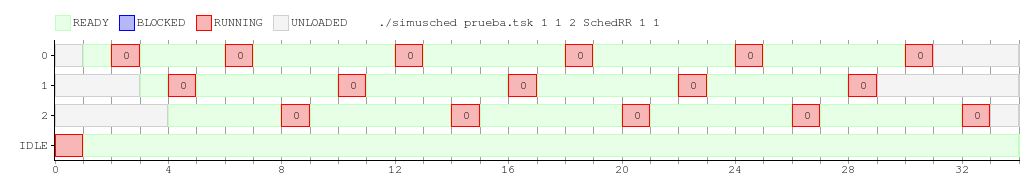
\includegraphics[width=1.1\textwidth]{img/salida_ej4_1.png}
     \caption{Experimentación de Round Robin}
\end{center}
\end{figure}

\textbf{Conclusiones:}

Los procesos se ejecutan de forma alternada, a medida que se van agregando a la lista de procesos \textit{ready}, y solo durante el quantum especificado.

\subsubsection{Segundo experimento:} 

En este segundo experimento utilizamos un lote con seis procesos. Tres procesos que utilizan intensivamente el CPU y tres procesos que realizan operaciones de E/S. El lote utilizado es el siguiente:

\begin{quote}
@1\\
TaskCPU 5\\
@2\\
TaskConsola 3 3 3\\
@3\\
TaskCPU 4\\
@4\\
TaskCPU 4\\
TaskConsola 2 4 4\\
@5\\
TaskConsola 1 5 5\\
\end{quote}

Fijamos en dos (2) la cantidad de núcleos del procesador, ya que con un solo núcleo no es posible observar que el scheduler realmente realiza migraciones de procesos entre núcleos, y con mas de dos núcleos no se obtiene ninguna información del scheduler que no se obtenga con dos núcleos.

A continuación, el gráfico resultante de ejecutar el lote de procesos con el scheduler Round-Robin:

\begin{figure}[H]
\begin{center}
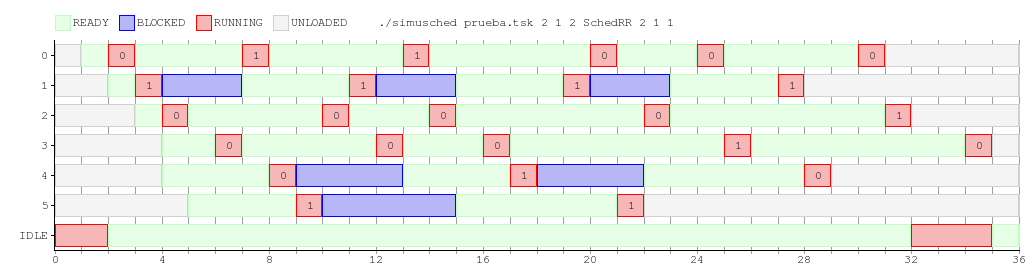
\includegraphics[width=1.1\textwidth]{img/salida_ej4_2.png}
     \caption{Experimentación de Round Robin}
\end{center}
\end{figure}

\textbf{Conclusiones:} 

Como se puede ver en el gráfico, los procesos se ejecutan en el primer núcleo que este libre independientemente de si se ejecuto previamente en ese núcleo o no, permitiendo así la migración de procesos entre núcleos.
También se puede ver que los procesos solo se ejecutan durante el quantum especificado y luego son desalojados para permitir a otro proceso utilizar el procesador.
Cuando un proceso se desbloquea o consume todo su quantum es añadido al final de la cola de procesos \textit{ready} lo cual, en muchos casos, altera el orden en el cual se ejecutan los procesos, es decir, los procesos no siempre se ejecutan en el orden en el cual llegaron.























\section{Pregunta 5}

\subsection{Enunciado del Problema:}

A partir del articulo
\begin{itemize}
	\item Waldspurger, C.A. and Weihl, W.E., Lottery scheduling: Flexible proportional-share re- source management. Proceedings of the 1st USENIX conference on Operating Systems Design and Implementation -1994.
\end{itemize}

disenar e implementar un scheduler basado en el esquema de loteria. El constructor de la clase SchedLottery debe recibir dos parametros: el quantum y la semilla de la secuencia pseudoaleatoria (en ese orden). Interesa implementar al menos la idea basica del algoritmo y la optimizacion de tickets compensatorios (compensation tickets). Otras optimizaciones y refinamientos que propone el articulo serian opcionales siempre que, en cada caso, se explique brevemente por que la optimizacion no se considero relevante a los efectos de este trabajo.
\subsection{Explicacion de la implementacion}
Para implementar \footnote{La implementacion de este scheduler se puede encontrar en el archivo \textit{sched\_lottery.cpp}.} esta política de scheduling utilizamos:
\begin{itemize}
	\item Un entero para llevar la cuenta de cuantos tickets hay en total entre todos los procesos \textit{ready}.
	\item Un diccionario donde la clave es el \textit{pid} del proceso y el valor es la cantidad de tickets que tiene dicho proceso. Solo los procesos \textit{ready} están definidos en esta estructura.
	\item Otro diccionario indexado por el \textit{pid} del proceso que permite sabe, en caso de que el proceso se haya bloqueado, cuantos ciclos de su \textit{quantum} utilizo.
\end{itemize}


Lo primero que hacemos es utilizar la semilla pasada como parámetro al constructor del scheduler para inicializar el generador de números pseudo-aleatorio con la función: \textit{srand(semilla)}.

Cada vez que un proceso se añade al scheduler, le otorgamos un valor constante de tickets \textit{(1000 tickets)}.
De esta forma, todos los procesos tienen, a priori, la misma probabilidad de ganar el uso del procesador.
Cuando un proceso gana el uso procesador, este lo tiene asignado durante un quantum \textit{(parámetro del scheduler)} y luego es desalojado.

Cuando un proceso se bloquea determinamos la cantidad \textbf{C} de ciclos del quantum asignado que utilizo, es decir, restar al Quantum del CPU la cantidad de ciclos utilizados por el proceso actual en el núcleo actual \textit{(este valor lo tenemos en un vector para cada núcleo)}.
Luego, cuando se desbloquea le otorgamos el \textit{compensation ticket} de forma que su cantidad total de tickets pasa a ser: $tickets$ $*$ $quantum$ $/$ $ciclosUtilizados$.
Cuando un proceso con un \textit{compensation ticket} gana el uso del procesador, pierde dicho ticket.

Para determinar cual es el proceso que gana el uso del procesador, llevamos a cabo una lotería entre todos los procesos \textit{ready}. Es decir, elegimos un numero al azar entre cero y la cantidad total de tickets entre todos los procesos \textit{ready}, este sera el ticket ganador. Luego, recorremos el diccionario que contiene a todos los procesos \textit{ready} sumando en un contador la cantidad de tickets de cada proceso hasta encontrar el proceso que hace que el valor de dicha sumatoria sea mayor o igual que el valor del ticket ganador. Este sera el proceso que ganara el uso del procesador, entonces restamos los tickets de este proceso de la cantidad de tickets total y lo eliminamos de la estructura que contiene a todos los procesos \textit{ready}.
\subsection{Pseudocodigo}


\begin{algorithm}[H]
\caption{SchedLottert(vector<int> argn)}
\label{pseudo:SchedLottery}
\begin{algorithmic}

\STATE BASE\_TICKETS = 1000
\STATE cores = argn[0]
\STATE cpuQuantum = argn[1]
\STATE semilla = argn[2]
\STATE srand(semilla)
\STATE quantumActual = Vector<int> de tamaño cores y cpuQuantum en cada posición;
\STATE procesos = Diccionario donde la clave es el pid del proceso y el valor asociado es la cantidad de tickets del proceso
\STATE bloqueados = Diccionario donde la clave es el pid del proceso y el valor asociado es la cantidad de ciclos de su quantum que utilizo antes de bloquearse;
\STATE ticketsTotales = 0

\end{algorithmic}
\end{algorithm}


\begin{algorithm}[H]
\caption{load(pid)}
\label{pseudo:load}
\begin{algorithmic}

\STATE load(pid, 0)

\end{algorithmic}
\end{algorithm}


\begin{algorithm}[H]
\caption{load(pid,deadline)}
\label{pseudo:loadD}
\begin{algorithmic}

\STATE procesos[pid] = BASE\_TICKETS
\STATE ticketsTotales = ticketsTotales + BASE\_TICKETS

\end{algorithmic}
\end{algorithm}



\begin{algorithm}[H]
\caption{unblock(pid)}
\label{pseudo:unblock}
\begin{algorithmic}

\STATE procesos[pid] = (BASE\_TICKETS * cpuQuantum / bloqueados[pid])
\STATE ticketsTotales = ticketsTotales + procesos[pid]

\end{algorithmic}
\end{algorithm}



\begin{algorithm}[H]
\caption{tick(cpu , Motivo m)}
\label{pseudo:tick}
\begin{algorithmic}

 \IF{(m == EXIT)}
	\IF{(procesos.vacio())}
		\STATE Devolver run\_idle\_task(cpu)
	\ELSE
		\STATE Devolver loteria(-1, cpu)	
	\ENDIF
	
\IF{(m == BLOCK)}
	\STATE bloqueados[current\_pid(cpu)] = cpuQuantum - quantumActual[cpu]
	\IF{(procesos.vacio())}
		\STATE Devolver run\_idle\_task(cpu)
	\ELSE
		\STATE Devolver loteria(-1, cpu)	
	\ENDIF
\ELSE
	\STATE quantumActual[cpu] = quantumActual[cpu] -1	
	\IF{(quantumActual[cpu] == 0)}
		\IF{(procesos.vacio())}
			\STATE Devolver current\_pid(cpu)
		\ELSE
			\STATE Devolver loteria(current\_pid(cpu), cpu)
		\ENDIF
	\ELSE
		\STATE Devolver current\_pid(cpu)
	\ENDIF
\ENDIF
\ENDIF
\end{algorithmic}
\end{algorithm}




\begin{algorithm}[H]
\caption{loteria(pid, cpu)}
\label{pseudo:loteria}
\begin{algorithmic}

\STATE quantumActual[cpu] = cpuQuantum

\IF{(pid != -1)}
	\STATE procesos[pid] = BASE\_TICKETS
	\STATE ticketsTotales = ticketsTotales + BASE\_TICKETS
\ENDIF

\STATE ticketGanador = rand() \% (ticketsTotales + 1)
\STATE procesoGanador = El pid de algún proceso
\STATE sumatoria = 0

\FOR{(Proceso p en procesos)}
\STATE sumatoria = sumatoria + p.tickets
\IF{(sumatoria $>=$ ticketGanador)}
	\STATE procesoGanador = p.pid
	\STATE Salir del for
\ENDIF

\ENDFOR

\STATE ticketsTotales = ticketsTotales - procesos[procesoGanador]
\STATE procesos.erase(procesoGanador)
\STATE Devolver procesoGanador
\end{algorithmic}
\end{algorithm}

\begin{algorithm}[H]
\caption{run\_idle\_task(cpu)}
\label{pseudo:runidletask}
\begin{algorithmic}
	\STATE quantumActual[cpu] = cpuQuantum
	\STATE devolver IDLE\_TASK
\end{algorithmic}
\end{algorithm}



\subsection{Optimizaciones propuestas por el articulo}

En el articulo se proponen algunas optimizaciones, a continuación nombramos cada una de ellas y el motivo por el cual fue o no fue implementada:
\begin{itemize}
	\item \textbf{Transferencia de tickets}: Esta optimizacion no la implementamos ya que,en el simulador utilizado, los procesos solo se bloquean a la espera de la E/S. Nunca se bloquean a la espera de otros procesos.
	\item \textbf{Inflación de tickets}: No nos pareció correcto que un proceso tenga la capacidad de otorgarse todos los tickets que desee, ya que de esta forma un proceso podría monopolizar el procesador. 
	\item \textbf{Tickets de compensación}: Fue implementado.
	\item \textbf{Ticket currencies}: Dado que los procesos, en el simulador, no tienen procesos hijos ni hay varios usuarios ejecutando procesos, no nos pareció necesario implementarlo. Ademas, seria imposible testear dicha implementacion.
	\item \textbf{Ordenar en forma decreciente la lista de procesos ready según la cantidad de tickets del proceso}: Esta es una optimizacion asintotica. Realmente harían falta muchos procesos para que tuviera un impacto notable, y por este motivo decidimos no implementarla.
\end{itemize}

\section{Pregunta 6}

\subsection{Enunciado del Problema:}

Programar un tipo de tarea TaskBatch que reciba dos parametros: total cpu y cant bloqueos. Una tarea de este tipo debera realizar cant bloqueos llamadas bloqueantes, en momentos elegidos pseudoaleatoriamente. En cada tal ocasion, la tarea debera permanecer bloqueada durante exactamente un (1) ciclo de reloj. El tiempo de CPU total que utilice una tarea TaskBatch deberia ser de total cpu ciclos de reloj (incluyendo el tiempo utilizado para lanzar las llamadas bloqueantes; no asi el tiempo en que la tarea permanezca bloqueada).
\subsection{Pseudocodigo}

\begin{algorithm}[H]
\caption{TaskBatch(pid,  params)}
\label{pseudo:TaskBatch}
\begin{algorithmic}

\STATE ciclosTotales = params[0]
\STATE entradasBloqueantes = params[1]
\STATE vector<int> ocupado(ciclosTotales,0)
\FOR{$i=0$ hasta $entradasBloqueantes$}
    \STATE momento = rand() \% ciclosTotales 
    \WHILE{ ocupado[momento]}
	\STATE momento = rand() \% ciclosTotales
    \ENDWHILE
    
    \STATE ocupado[momento] = 1
\ENDFOR

\FOR{$i=0$ hasta $ciclosTotales$}
\IF{(ocupado[i])}
	\STATE uso\_IO(pid, 1)
\ELSE
	\STATE uso\_CPU(pid, 1)
\ENDIF
\ENDFOR
\end{algorithmic}
\end{algorithm}

\subsection{Explicación de la implementacion}

Se crea un vector de tamaño $ciclosTotales$ (es la cantidad total de ciclos de uso de CPU de la tarea) inicializado en cero. Lo interpretaremos como un vector de booleanos, donde si la posición i esta en 1, es porque en el momento i se hace una llamada bloqueante y cero en caso de que sea un ciclo solo de uso de CPU. Al principio en todas los momentos se esta usando solo CPU.

Luego se itera $entradasBloqueantes$ (es la cantidad de llamadas bloqueantes en la tarea) veces y se elije un momento al azar entre 0 y $ciclosTotales$. Si ese momento ya estaba ocupado ($ocupado[momento] = TRUE$) entonces se vuelve a elegir al azar para tomar otro momento. Luego se setea en uno indicando que habrá una llamada bloqueante en ese momento.

Luego se recorre el vector y se ejecuta la tarea. Si el $ocupado[momento] = TRUE$ entonces se ejecuta un ciclo de uso de CPU y una llamada bloqueante, sino se ejecuta un solo ciclo de CPU.
\section{Pregunta 7}

\subsection{Enunciado del Problema:}

Disenar un lote de tareas TaskBatch, todas ellas con igual uso de CPU, pero con diversas cantidades de bloqueos. Simular este lote utilizando el algoritmo SchedRR y una variedad apropiada de valores de quantum. Mantener fijo en un (1) ciclo de reloj el costo de cambio de contexto y dos (2) ciclos el de migracion. Deben variar la cantidad de nucleos de procesamiento. Para cada una de las metricas elegidas, concluir cual es el valor optimo de quantum a los efectos de dicha metrica.

Elegimos 2 métricas para analizar las tareas TaskBatch: Turnarround y Waiting time.

Turnarround es una métrica que analiza cuanto tarda un proceso en terminar (en promedio), se puede usar para analizar el tiempo de ejecución de un programa en promedio.

Waiting time analiza el tiempo en que un proceso esta en la cola de listos en su vida, se usa para analizar lo que tiene que esperar un proceso para ejecutarse y también el tiempo en que no esta haciendo nada.

Usamos el scheduling Round Robin con costo 1 en cambio de contexto y 2 en migración entre núcleos. 

Para los gráficos, realizamos un lote de 5 tareas batch dejando fijo la cantidad de ciclos totales para las tareas en 10 y variando entre 1,2,3,4 y 5 llamadas bloqueantes para cada proceso (en ese orden).

En los primeros graficos dejamos fijo la cantidad de cores en 1 y variamos el quantum en cada uno en 1,3,6,9,10. Calculamos para cada uno Turnarround y Waiting time.

El Turnarround lo calculamos dividiendo $\frac{ciclosP_0 + ciclosP_1 + ciclosP_2 + ciclosP_3 + ciclosP_4 }{5}$. Eso nos devuelve la cantidad de ciclos que le toma a un proceso en ejecutarse en promedio.

El Waiting time se calcula tomando el promedio de tiempo de espera de cada proceso, cuyo valor se calcula sumando los ciclos en donde el proceso esta en la cola de listos.

\subsection{Experimento con 1 core}

\begin{figure}[H]
\begin{center}
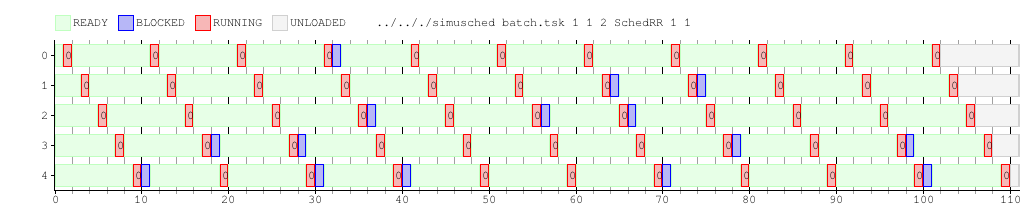
\includegraphics[width=1.1\textwidth]{img/core1q1.png}
     \caption{Round Robin con quantum 1}
\end{center}
\end{figure}

Turnarround: 105 ciclos

Waiting time: 92 ciclos 

\begin{figure}[H]
\begin{center}
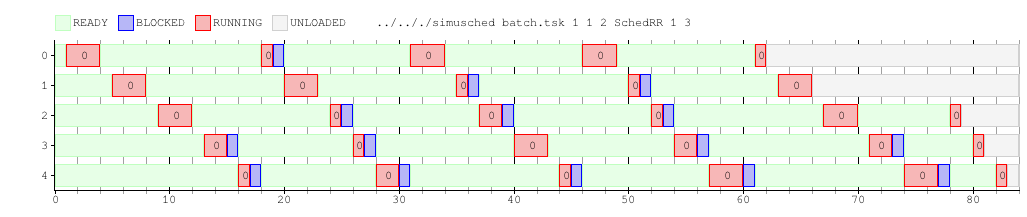
\includegraphics[width=1.1\textwidth]{img/core1q3.png}
     \caption{Round Robin con quantum 3}
\end{center}
\end{figure}

Turnarround: 74.2 ciclos

Waiting time: 60.2 ciclos 

\begin{figure}[H]
\begin{center}
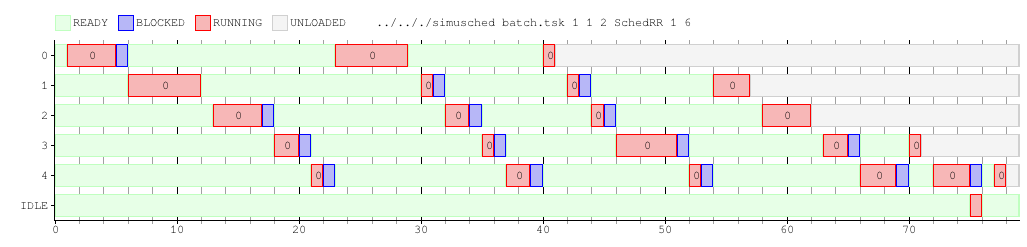
\includegraphics[width=1.1\textwidth]{img/core1q6.png}
     \caption{Round Robin con quantum 6}
\end{center}
\end{figure}

Turnarround: 62.8 ciclos

Waiting time: 47.8 ciclos 

\begin{figure}[H]
\begin{center}
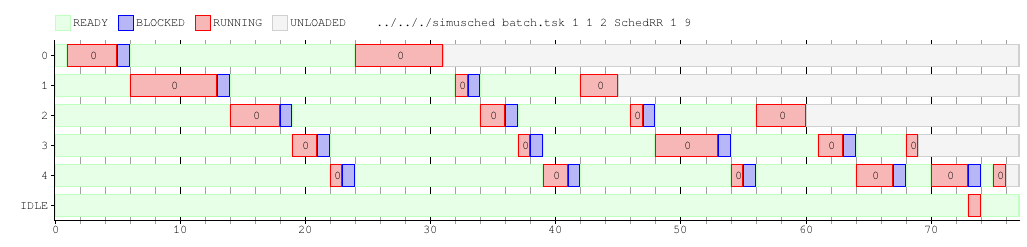
\includegraphics[width=1.1\textwidth]{img/core1q9.png}
     \caption{Round Robin con quantum 9}
\end{center}
\end{figure}

Turnarround: 56.2 ciclos

Waiting time: 42.2 ciclos 

\begin{figure}[H]
\begin{center}
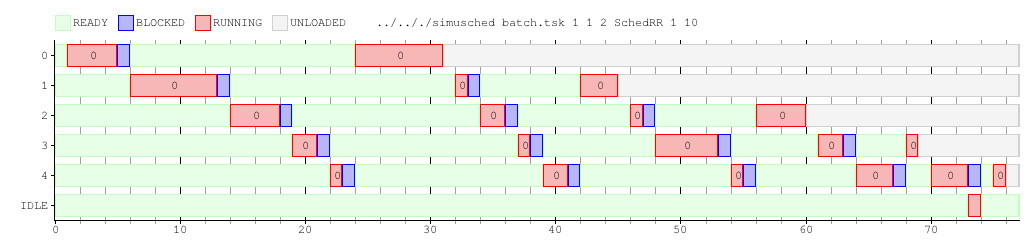
\includegraphics[width=1.1\textwidth]{img/core1q10.png}
     \caption{Round Robin con quantum 10}
\end{center}
\end{figure}

Turnarround: 56.2 ciclos

Waiting time: 42.2 ciclos 

\begin{figure}[H]
\begin{center}
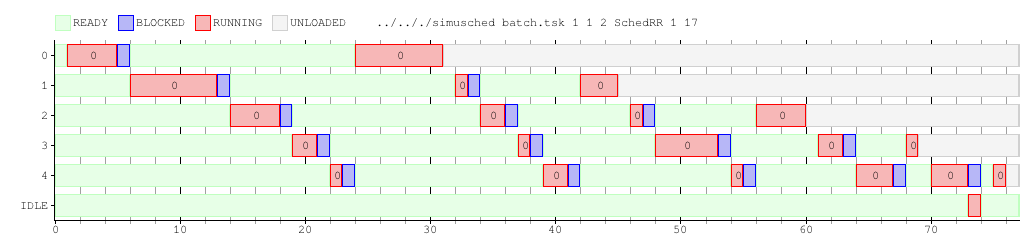
\includegraphics[width=1.1\textwidth]{img/core1q17.png}
     \caption{Round Robin con quantum 17}
\end{center}
\end{figure}

Turnarround: 56.2 ciclos

Waiting time: 42.2 ciclos

Como se puede observar ambas métricas mejoran mientras en quantum es mas alto, pero luego de tener quantum 9, las métricas dan lo mismo (por dar el mismo gráfico). Por lo tanto el valor óptimo de quantum es 9 para este tipo de test.

\subsection{Experimento con 2 cores}

\begin{figure}[H]
\begin{center}
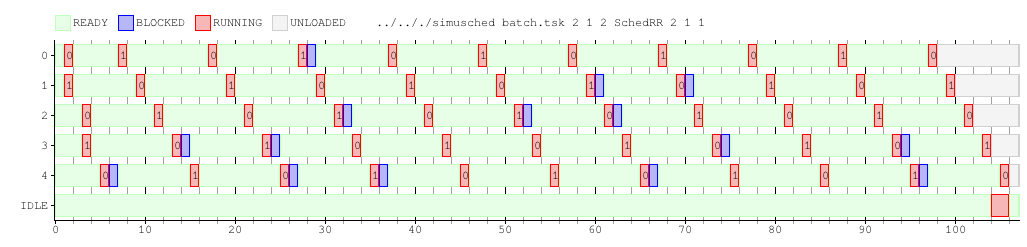
\includegraphics[width=1.1\textwidth]{img/core2q1.png}
     \caption{Round Robin con quantum 1}
\end{center}
\end{figure}

Turnarround: 102 ciclos

Waiting time: 88 ciclos 

\begin{figure}[H]
\begin{center}
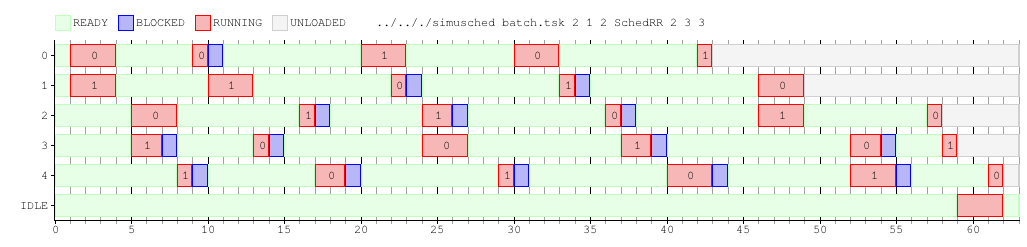
\includegraphics[width=1.1\textwidth]{img/core2q3.png}
     \caption{Round Robin con quantum 3}
\end{center}
\end{figure}

Turnarround: 54.4 ciclos

Waiting time: 40.2 ciclos 

\begin{figure}[H]
\begin{center}
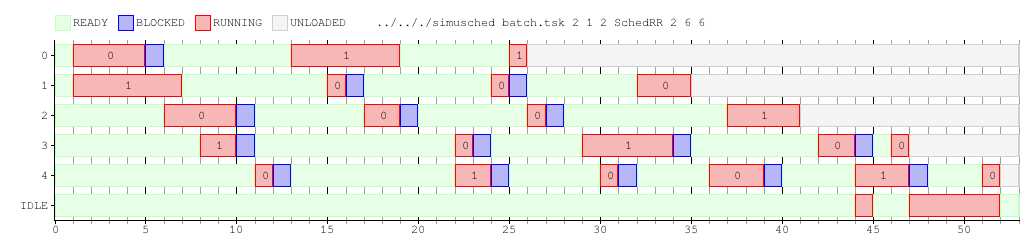
\includegraphics[width=1.1\textwidth]{img/core2q6.png}
     \caption{Round Robin con quantum 6}
\end{center}
\end{figure}

Turnarround: 40.2 ciclos

Waiting time: 26.2 ciclos 

\begin{figure}[H]
\begin{center}
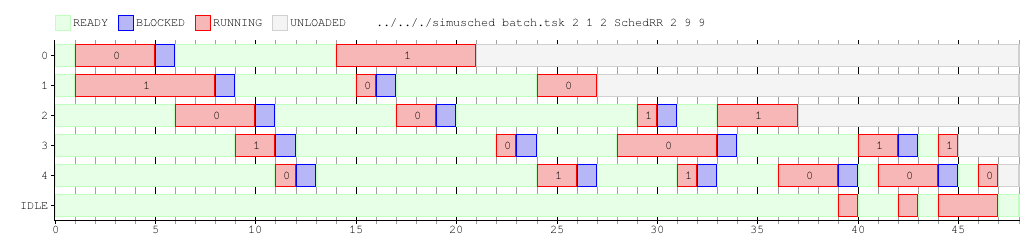
\includegraphics[width=1.1\textwidth]{img/core2q9.png}
     \caption{Round Robin con quantum 9}
\end{center}
\end{figure}

Turnarround: 35.4 ciclos

Waiting time: 21.4 ciclos 

\begin{figure}[H]
\begin{center}
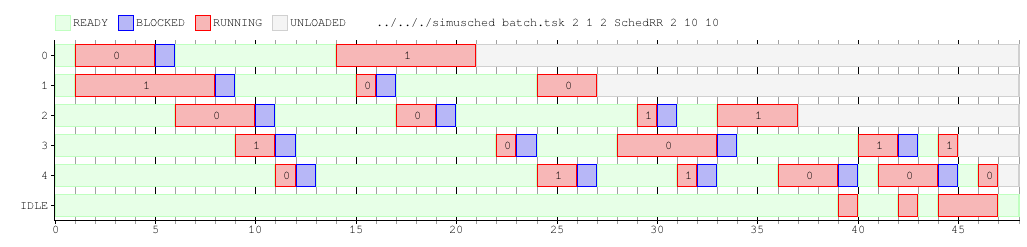
\includegraphics[width=1.1\textwidth]{img/core2q10.png}
     \caption{Round Robin con quantum 10}
\end{center}
\end{figure}

Turnarround: 35.4 ciclos

Waiting time: 21.4 ciclos 

\begin{figure}[H]
\begin{center}
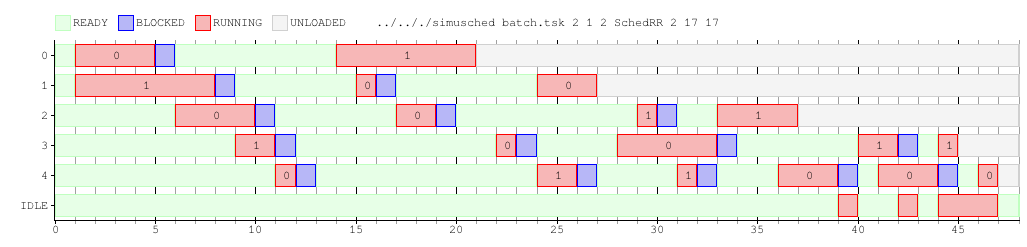
\includegraphics[width=1.1\textwidth]{img/core2q17.png}
     \caption{Round Robin con quantum 17}
\end{center}
\end{figure}

Turnarround: 56.2 ciclos

Waiting time: 42.2 ciclos

Como se puede observar ambas métricas mejoran mientras en quantum es mas alto, pero luego de tener quantum 9, las métricas dan lo mismo (por dar el mismo gráfico). Por lo tanto el valor óptimo de quantum es 9 para este tipo de test.

\subsection{Experimento con 4 cores}

\begin{figure}[H]
\begin{center}
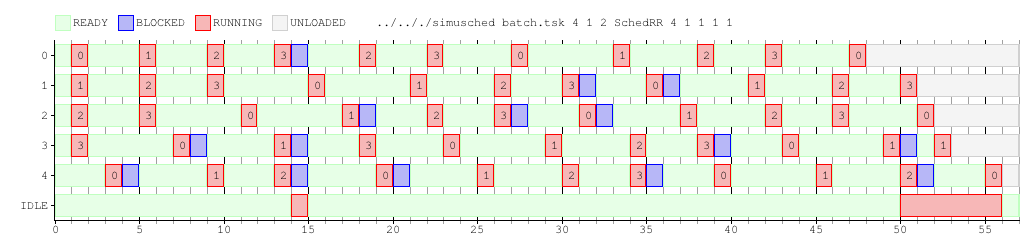
\includegraphics[width=1.1\textwidth]{img/core4q1.png}
     \caption{Round Robin con quantum 1}
\end{center}
\end{figure}

Turnarround: 51 ciclos

Waiting time: 38 ciclos 

\begin{figure}[H]
\begin{center}
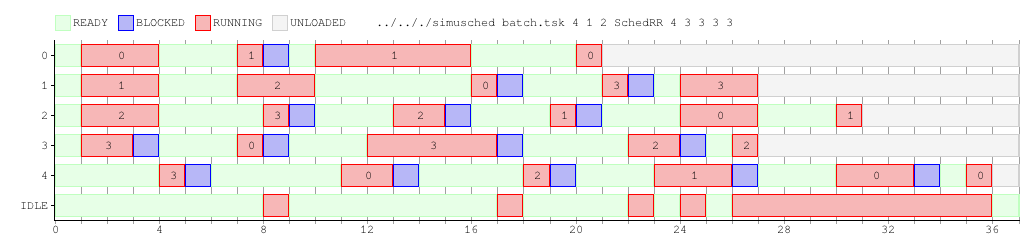
\includegraphics[width=1.1\textwidth]{img/core4q3.png}
     \caption{Round Robin con quantum 3}
\end{center}
\end{figure}

Turnarround: 28.4 ciclos

Waiting time: 14.4 ciclos 

\begin{figure}[H]
\begin{center}
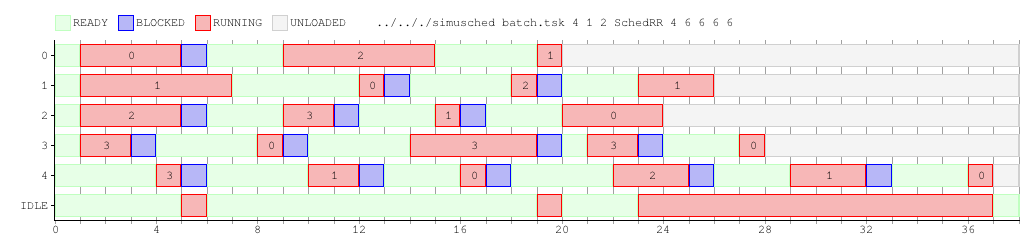
\includegraphics[width=1.1\textwidth]{img/core4q6.png}
     \caption{Round Robin con quantum 6}
\end{center}
\end{figure}

Turnarround: 27 ciclos

Waiting time: 13 ciclos 

\begin{figure}[H]
\begin{center}
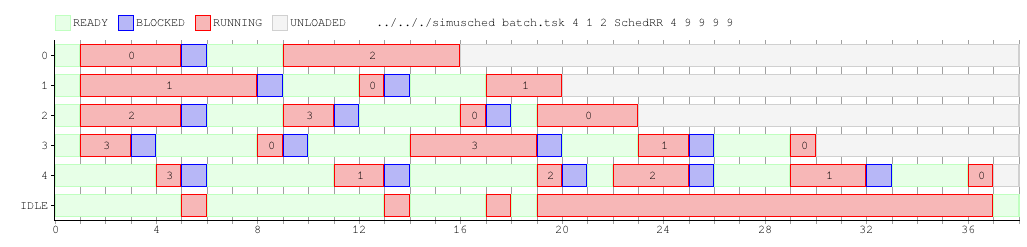
\includegraphics[width=1.1\textwidth]{img/core4q9.png}
     \caption{Round Robin con quantum 9}
\end{center}
\end{figure}

Turnarround: 25 ciclos

Waiting time: 10.2 ciclos 

\begin{figure}[H]
\begin{center}
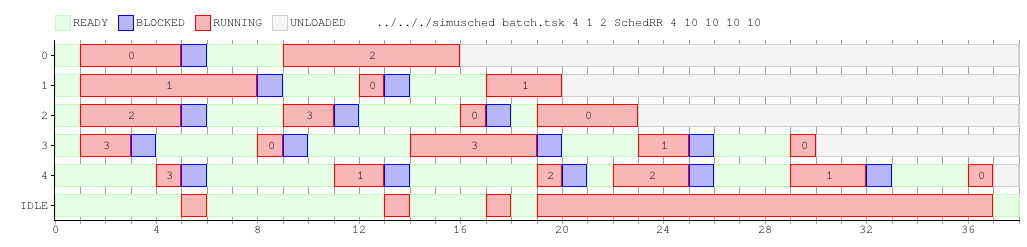
\includegraphics[width=1.1\textwidth]{img/core4q10.png}
     \caption{Round Robin con quantum 10}
\end{center}
\end{figure}

Turnarround: 25 ciclos

Waiting time: 10.2 ciclos 

\begin{figure}[H]
\begin{center}
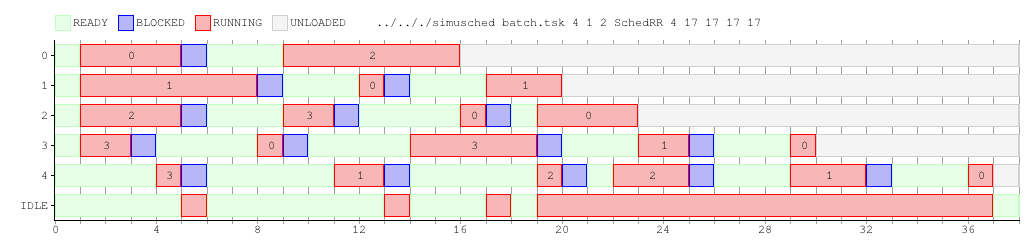
\includegraphics[width=1.1\textwidth]{img/core4q17.png}
     \caption{Round Robin con quantum 17}
\end{center}
\end{figure}

Turnarround: 56.2 ciclos

Waiting time: 42.2 ciclos

Como se puede observar ambas métricas mejoran mientras en quantum es mas alto, pero luego de tener quantum 9, las métricas dan lo mismo (por dar el mismo gráfico). Por lo tanto el valor óptimo de quantum es 9 para este tipo de test.
\section{Pregunta 8}

\subsection{Enunciado del Problema:}

Implemente un scheduler Round-Robin que no permita la migración de procesos entre núcleos (SchedRR2). La asignación de CPU se debe realizar en el momento en que se produce la carga de un proceso (load). El nucleo correspondiente a un nuevo proceso sera aquel con menor cantidad de procesos activos totales (RUNNING + BLOCKED + READY). Disene y realice un conjunto de experimentos que permita evaluar comparativamente las dos implementaciones de Round-Robin.

\subsection{Explicación de la implementacion}

Para implementar esta política de scheduling utilizamos las siguientes estructuras:
\begin{itemize}
	\item Un vector para almacenar el valor del quantum de cada núcleo del procesador.
	\item Un vector que contiene la cola de procesos \textit{ready} de cada núcleo.
	\item Un vector que almacena cuantos procesos bloqueados hay en cada núcleo.
	\item Un diccionario que indica a que núcleo esta asignado cada proceso.
\end{itemize}

Cada vez que un proceso se añade al scheduler calculamos, para cada núcleo, la cantidad de procesos activos, es decir: $RUNNING\ +\ BLOCKED\ +\ READY$. El núcleo con tenga el menor valor en dicha suma sera el núcleo asignado al nuevo proceso.
Entonces, en el diccionario añadimos una entrada para la clave del \textit{pid} del proceso y como valor colocamos el núcleo elegido. De esta forma siempre sabemos a que núcleo fue asignado el proceso.

Cuando un proceso se bloquea, incrementamos en uno el contador de procesos bloqueados del núcleo en el que el proceso se ejecuto. Cuando se desbloquea, lo disminuimos en uno y colocamos el proceso en la cola de procesos \textit{ready} del núcleo que se le asigno al ser cargado.

Cuando debemos determinar el próximo proceso a ejecutar en un núcleo, simplemente tomamos el primer elemento de la cola de procesos \textit{ready} correspondiente a dicho núcleo.

\subsection{Comparación entre los algoritmos de Round Robin}

En todas las pruebas subsecuentes utilizamos la siguiente configuración del simulador:
\begin{itemize}
	\item \textbf{Dos (2) núcleos}. Ya que con un solo núcleo los algoritmos se comportarían exactamente igual y con dos núcleos ya es posible mostrar las diferencias en el comportamiento.
	\item \textbf{Costo de cambio de contexto}: Un (1) ciclo de reloj.
	\item \textbf{Costo de migración de núcleo}: Dos (2) ciclos de reloj.
	\item \textbf{Quantum de cada núcleo}: Dos (2) ciclos de reloj.
\end{itemize}

\subsubsection{Primer experimento}

En este primer experimento solo ejecutamos tareas que utilizan intensivamente el CPU durante diferente tiempo. El lote utilizado es el siguiente:

\begin{quote}
@1\\
TaskCPU 15\\
@3\\
TaskCPU 5\\
TaskCPU 15\\
@4\\
TaskCPU 2
\end{quote}

El resultado de utilizar RR y RR2 fue:

\begin{figure}[H]
\begin{center}
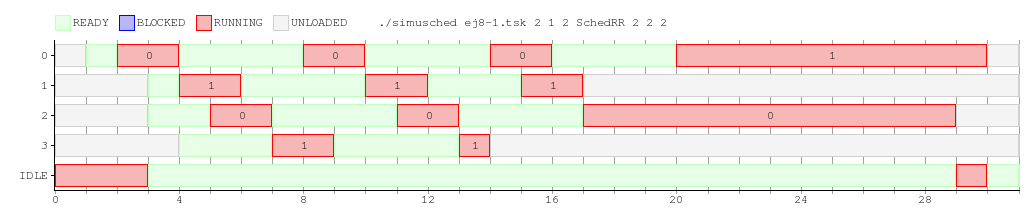
\includegraphics[width=1.1\textwidth]{img/ej8-1-RR.png}
     \caption{Round Robin con migración entre núcleos}
\end{center}
\end{figure}

\begin{figure}[H]
\begin{center}
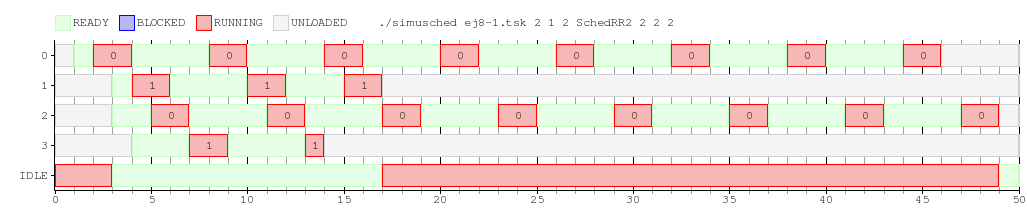
\includegraphics[width=1.1\textwidth]{img/ej8-1-RR2.png}
     \caption{Round Robin sin migración entre núcleos}
\end{center}
\end{figure}

Como se puede observar en los gráficos, la migración entre núcleos permite al primer scheduling terminar mucho mas rápido \textit{(20 ciclos antes, aunque esta diferencia podría ser arbitrariamente grande)} que el segundo, que no permite migrar procesos entre núcleos.
Esto se debe a que, en el segundo scheduler, se asigna el núcleo cero a las dos tareas mas largas \textit{(tareas 0 y 2)}. Entonces, al no estar permitida la migración entre núcleos, el núcleo cero debe ejecutar ambas tareas mientras el núcleo uno esta ocioso \textit{(lo cual es algo totalmente indeseado)}.

\subsubsection{Segundo experimento}

En el segundo experimento utilizamos tareas que utilizan intensivamente la E/S.
El lote utilizado fue el siguiente:

\begin{quote}
@1\\
TaskConsola 6 3 3\\
@3\\
TaskConsola 5 5 5\\
TaskConsola 4 7 7\\
@4\\
TaskConsola 6 4 4\\
\end{quote}

El resultado de utilizar RR y RR2 fue:

\begin{figure}[H]
\begin{center}
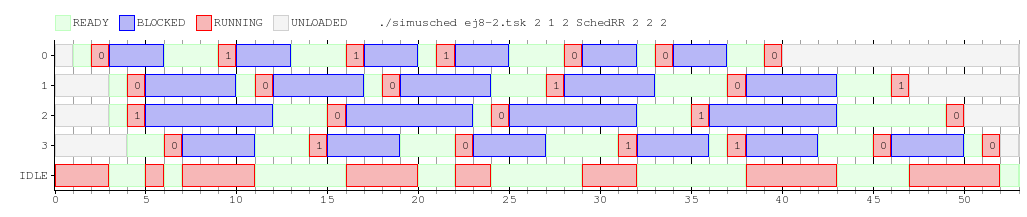
\includegraphics[width=1.1\textwidth]{img/ej8-2-RR.png}
     \caption{Round Robin con migración entre núcleos}
\end{center}
\end{figure}

\begin{figure}[H]
\begin{center}
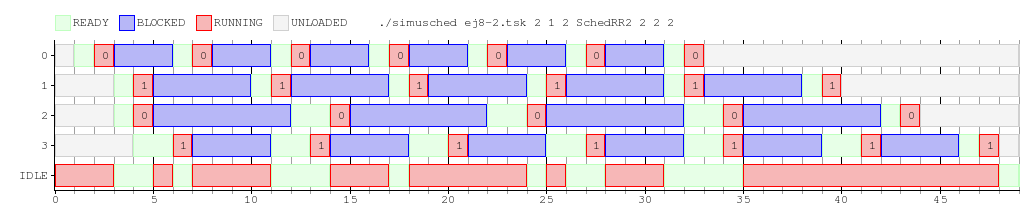
\includegraphics[width=1.1\textwidth]{img/ej8-2-RR2.png}
     \caption{Round Robin sin migración entre núcleos}
\end{center}
\end{figure}

Como se puede ver en los gráficos, en este caso el scheduler Round Robin que no permite la migración entre núcleos termina antes que el si lo permite. Esto es debido a que el costo de migrar un proceso de un núcleo a otro es mayor que el costo que tendría esperar a que el núcleo que se le asigno previamente quede libre, pues las tareas se bloquean muy rápidamente.

\subsubsection{Conclusión}

En algunos casos, puede resultar beneficioso que un proceso espere al núcleo que tenia asignado previamente antes que realizar un migración. Pero, si dicho núcleo no se libera rápidamente y, ademas, teníamos otro núcleo libre, hubiera sido mejor pagar el costo de una migración entre núcleos.

En el primer experimento solo teníamos una tarea a la espera de que su núcleo asignado se libere, mientras había otro núcleo libre. Pero, fácilmente, podría generarse un escenario donde la cantidad de procesos a la espera de un núcleo sea arbitrariamente grande y que la cantidad de núcleos libres también sea arbitrariamente grande, dando como resultado una asignación muy ineficiente de los recursos disponibles.

Por lo dicho, podemos concluir que permitir la migración entre núcleos es, en la mayoría de los casos, mas conveniente que prohibirlo.

\section{Pregunta 9}

\subsection{Enunciado del Problema:}

Disenar y llevar a cabo un experimento que permita poner a prueba la ecuanimidad (fairness) del algoritmo SchedLottery implementado. Tener en cuenta que, debido al factor pseudoaleatorio involucrado, cualquier corrida puntual podria ser arbitrariamente injusta; sin embargo, si se repite un mismo experimento n veces y se observan los resultados acumulativos, tales anomalias deberian ir desapareciendo conforme n aumenta. En otras palabras, interesa mostrar en base a evidencia empirica que el algoritmo implementado efetivamente tiende a ser totalmente ecuanime a medida que n tiende a infinito.


\subsubsection{Introducción}

Para poner a prueba la ecuanimidad (fairness) del \textit{Lottery Scheduling} fijaremos los siguiente parámetros:
\begin{itemize}
	\item Quantum de 4 ciclos de clock. Este valor no afecta la ecuanimidad.
	\item Costo de cambio de contexto y de migración entre núcleos: 0 ciclos de clock, para que no entorpezca las mediciones y, ademas, es un valor que no afecta el \textit{fairness}.
\end{itemize}

La experimentación la realizamos con uno y dos núcleos de procesamiento, para ver si el \textit{fairness} se da en ambos casos.\\


Vamos a utilizar tanto tareas que utilizan intensivamente el CPU como tareas que utilizan la E/S. El lote de tareas elegido es el siguiente:
\begin{quote}
TaskCPU 25\\
TaskCPU 22\\
TaskBatch 14 7\\
TaskBatch 12 9\\
TaskConsola 10 2 2\\
\end{quote}

Elegimos este lote para tener variedad tanto en el tiempo de ejecución de los procesos como en el uso de la CPU y de la E/S que estos realizan.\\


La métrica elegida para medir el \textit{fairness} es \textit{promedio del uso del CPU por tiempo de espera de cada proceso}, es decir, llevamos a cabo la siguiente cuenta para determinar el valor de la métrica en un experimento:
\begin{itemize}
	\item Para cada proceso $i$ calculamos cuantos ciclos del CPU utilizo el proceso, lo llamamos $CPU_i$ y cuanto tiempo espero, lo llamamos $T_i$.
	\item Luego, el valor de la métrica para el experimento es: $\frac{1}{n}$ $*$ $\sum_{i = 1}^{n} \frac{CPU_i}{T_i}$
\end{itemize}


El concepto de \textit{fairness} en el lottery scheduling es:

\begin{itemize}

	\item Cuanto menos usa de su quantum un proceso antes de bloquearse, mas probable es que el proceso gane el CPU \textit{pronto} (ya que se le otorga un \textit{compensation ticket}), es decir, que a menor uso del quantum menor debería ser el tiempo de espera antes de volver a tener el CPU.

	\item Si un proceso utiliza todo su quantum, es probable que deba esperar mas tiempo que los procesos que solo utilizan una fracción de este, es decir, a mayor uso del CPU mayor debería ser el tiempo de espera antes de volver a tener el CPU.

\end{itemize}

Luego, si \textbf{en promedio} todos los procesos tienen un relación similar entre el uso del CPU y el tiempo que esperan (a lo largo de los experimentos) podríamos decir que el \textit{lottery scheduling} es justo asignando el CPU.
Justamente, la métrica elegida nos permite ver esta relación.\\

Es importante señalar que la métrica utilizada no se ve afectada por el tiempo que el proceso esta bloqueado, ya que los dos valores que determinan su valor (uso del CPU y tiempo de espera) son independientes del tiempo que el proceso esta bloqueado.\\


En cada conjunto de experimentos, decidimos llevar a cabo la medición de la métrica hasta un determinado tick del procesador que nos garantice que aun no haya terminado de ejecutarse ningún proceso (es decir, que todos compiten por el CPU) y, ademas, independiza la experimentación de los tiempos de ejecución totales de los procesos en el lote de procesos.

\subsubsection{Experimentación con un núcleo}

A continuación los resultados de la experimentación realizada utilizando diferentes semillas para el generador de números aleatorios.

Para cada experimento, calculamos la métrica para cada proceso, es decir, el valor $\frac{CPU_i}{T_i}$ y la métrica para el experimento, es decir, el promedio de los valores anteriores.

En este experimento decidimos llevar a cabo la medición hasta el tick numero 40 del procesador que, como dijimos antes, nos garantiza que ningún procesos haya terminado.
A continuación, los resultados de la experimentación realizada:

\begin{figure}[H]
\begin{center}
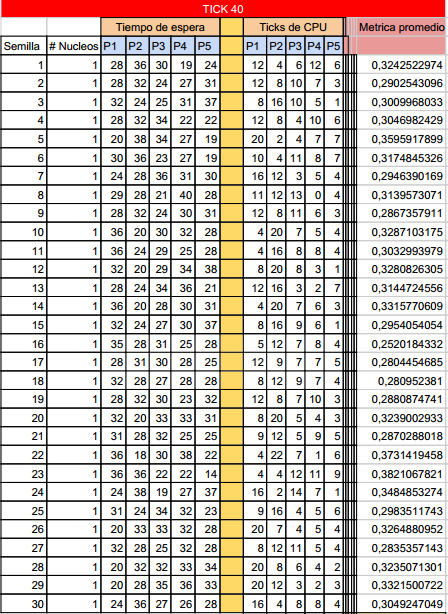
\includegraphics[width=0.7\textwidth]{img/foto1.png}
     \caption{Lottery Scheduling con un solo núcleo hasta el tick 40}
\end{center}
\end{figure}


Como puede apreciarse en la tabla, la métrica da valores muy similares para todos los experimentos realizados.
Para ver que relación existe entre estos valores calculamos la varianza, la esperanza y el desvió estándar de la muestra, lo cuales se definen como:
\begin{center}
	Esperanza $=$ $\mu$ $=$ $\bar{X}$ $=$ $\frac{1}{n}$ $*$ $\sum_{i = 1}^{n}(X_i)$\\
	Varianza $=$ $\sigma^{2}$ $=$ $\frac{1}{n}$ $*$ $\sum_{i = 1}^{n} (X_i - \bar{X})^{2}$\\
	Desvió estandar $=$ $\sigma$ $=$ $\sqrt{Varianza}$	
\end{center}

\begin{figure}[H]
\begin{center}
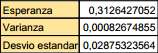
\includegraphics[width=0.4\textwidth]{img/img3.png}
     \caption{Esperanza, varianza y desvió estándar de la métrica promedio}
\end{center}
\end{figure}

Como se puede ver, la varianza y el desvió estándar son muy chicos en comparación con la esperanza.
Numéricamente hablando, la varianza es un $0.26\%$ de la esperanza y el desvió estándar es un $9.20\%$ de la esperanza.

Entonces, como el valor esperado (i.e esperanza) de la métrica se encuentra dentro de un intervalo muy pequeño $(\mu - \sigma, \mu + \sigma)$ $=$ $(0.28,$ $0.34)$, podemos concluir, en base a la experimentación realizada y a la métrica utilizada, que este mismo comportamiento ocurrirá en la mayoría de los experimentos y que, por lo tanto, el \textit{Lottery scheduling} es justo.



\subsubsection{Experimentación con dos núcleos}

En este experimento decidimos llevar a cabo la medición hasta el tick numero 25 del procesador, por los motivos ya dichos anteriormente.
A continuación, los resultados de la experimentación realizada:


\begin{figure}[H]
\begin{center}
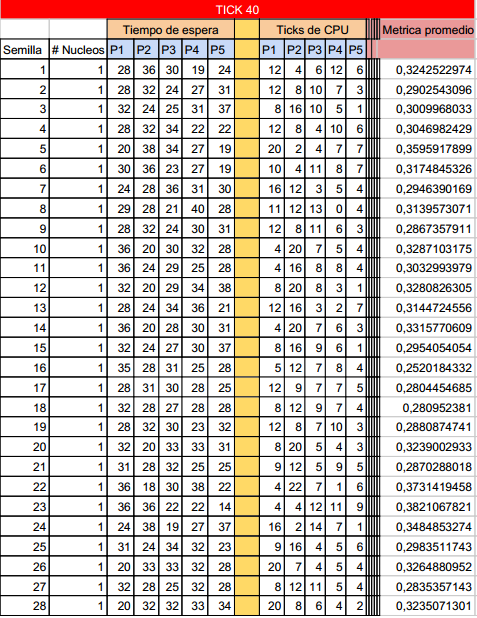
\includegraphics[width=0.6\textwidth]{img/fotaza1.png}
     \caption{Lottery Scheduling con un dos núcleos hasta el tick 25}
\end{center}
\end{figure}

Al igual que sucedió en la experimentación de un solo núcleo, los valores obtenidos con la métrica son muy similares.
Para ver que relación hay entre estos vamos a calcular nuevamente, la esperanza, la varianza y el desvió estándar de la muestra.
Los resultados obtenidos son los siguientes:
\begin{figure}[H]
\begin{center}
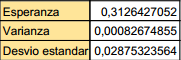
\includegraphics[width=0.4\textwidth]{img/fotaza2.png}
     \caption{Esperanza, varianza y desvió estándar de la métrica promedio}
\end{center}
\end{figure}

Como se puede ver, la varianza es un $2.75\%$ de la esperanza y el desvió estándar es un $15.75\%$ de la esperanza y, el desvió estándar, nos dice que la esperanza se encuentra en el intervalo $(\mu - \sigma, \mu + \sigma)$ $=$ $(0.93$, $1.28)$.
Por esto y por el hecho de que el intervalo en el que se encuentra la esperanza es pequeño, podemos suponer que el resultado obtenido en la experimentación realizada se repetirá en la mayoría de los casos y que, en consecuencia, el \textit{Lottery scheduling} es justo.

\subsubsection{Conclusión}

En general, el Lottery Scheduling se comporta de forma ecuánime, como podemos ver en los experimentos, ya que los intervalos de la esperanza son muy pequeños con ambos núcleos y la varianza también es pequeña. Por otro lado por el factor aleatorio de este algoritmo, es posible que se den casos extremos en donde una tarea o proceso es pospuesto por mucho tiempo o que una tarea gane el uso del CPU muy seguido.
\section{Pregunta 10}

\subsection{Enunciado del Problema:}
Los autores del articulo sobre lottery scheduling alegan que la optimizacion de compensation tickets es necesaria para compensar una posible falencia del algoritmo inicialmente propuesto en ciertos escenarios. Disenar y llevar a cabo un experimento apropiado para comprobar esta afirmacion (provocar un escenario donde se manifieste el problema, comparar simulaciones ejecutadas con y sin compensation tickets y discutir los resultados obtenidos).

\subsection{Solución}
Dado que lo que queremos ver es que la optimizacion de \textit{Compensation tickets} es necesaria, mostraremos que en un escenario propuesto por nosotros el \textit{lottery scheduling} es menos justo con la asignación del CPU a los procesos si no utiliza el \textit{compensation ticket}.

El escenario propuesto es el siguiente:
\begin{itemize}
	\item Fijaremos el quantum en 4 ciclos de clock.
	\item Fijaremos el costo de cambio de contexto y el costo de cambio de núcleo en cero ciclos de clock para que no entorpezcan las mediciones.
	\item Fijaremos el numero de núcleos de procesamiento en uno.
\end{itemize}


Ademas, utilizaremos el siguiente lote de tareas:
\begin{quote}
TaskCPU 35\\
TaskCPU 35\\
TaskBatch 9 9\\
\end{quote}


Elegimos este lote para tener dos procesos que utilizan intensivamente el CPU compitiendo continuamente por el CPU y que, al deshabilitar el \textit{Compensation Ticket}, obliguen al proceso TaskBatch a esperar mucho antes de poder utilizar el CPU.

Ademas, cada vez que el proceso TaskBatch gane el CPU, lo utilizara por un solo ciclo y luego se bloqueara (por como esta implementado TaskBatch).
Se hace eligio esto para minimizar la cantidad de quantum que la tareas bloqueante utiliza y así maximizar la cantidad de tickets que obtendrá el proceso por los Compensation Tickets.\\

Es importante señalar que probamos con muchos otros lotes de tareas y, en todos ellos, obteníamos el resultado inverso al esperado, es decir, la experimentación daba como resultado que el algoritmo sin compensation ticket era mas justo que con.
Con este lote de tareas no sucede eso, y ese fue otro de los motivos por el cual lo elegimos.

Utilizaremos la métrica descrita en el \textbf{Ejercicio 9} para medir el \textit{fairness} del algoritmo, y llevaremos a cabo la medición hasta el tick 42 del procesador, por los motivos que explicamos en el ejercicio anterior.\\


A continuación, exponemos los resultados de la experimentación utilizando el Compensation Ticket y el lote descrito:


\begin{figure}[H]
\begin{center}
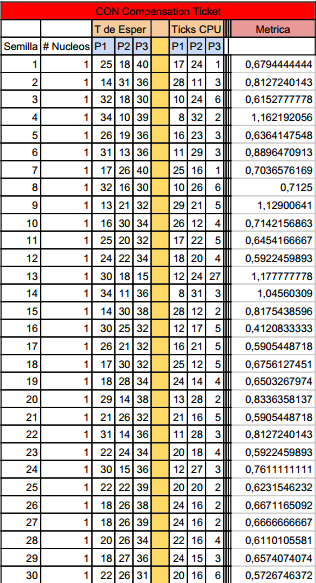
\includegraphics[width=0.6\textwidth]{img/refotaza1.png}
     \caption{Lottery Scheduling con Compensation Tickets hasta el tick 42}
\end{center}
\end{figure}

Ahora, si llevamos a cabo la misma experimentación, pero \textbf{sin Compensation Ticket} resulta en el siguiente gráfico:

\begin{figure}[H]
\begin{center}
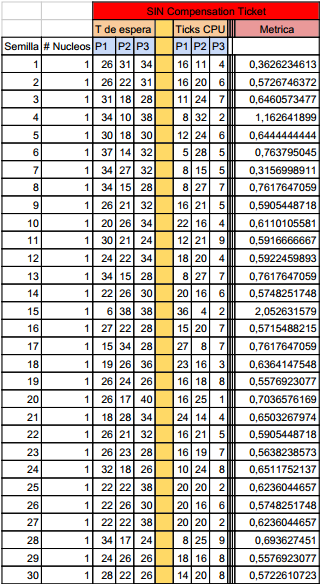
\includegraphics[width=0.6\textwidth]{img/refotaza2.png}
     \caption{Scheduling lottery sin Compensation Tickets hasta el tick 42}
\end{center}
\end{figure}


Ahora, para comparar los resultados obtenidos en ambos experimentos, calcularemos la esperanza, la varianza y el desvió estándar de ambas muestras.
El resultado es el siguiente:
\begin{figure}[H]
\begin{center}
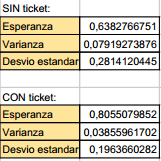
\includegraphics[width=0.3\textwidth]{img/refotaza3.png}
     \caption{Esperanza, Varianza, y Desvió estándar de las muestras}
\end{center}
\end{figure}

Como se puede observar, tanto la varianza como el desvió estándar son mayores cuando el algoritmo no utiliza el Compensation Ticket, es decir, el intervalo en el cual se haya la esperanza $(\mu - \sigma, \mu + \sigma)$ es mayor y, por lo tanto, podemos concluir que el algoritmo es menos justo asignando el CPU.
Luego, podemos concluir que en ciertos escenarios, la optimizacion del Compensation Ticket es necesaria, pues sin el Compensation ticket la asignación del CPU es menos justa.


\newpage

\end{document}



